\subsubsection{Digitiztaion of the Hadronic Veto System (Editors: Nhan Tran, Andrew Whitbeck)}
\label{sec:hcaldig}

After full {\tt GEANT4} simulation, we simulate the digitization of the particle-level interactions in our detector to understand how well we can reconstruct events in the hadronic calorimeter.
Given the particle-level energy deposition per layer, we can convert that into the number of minimum ionizing particles (MIP) that we expect in that layer.
The translation comes by first estimating the typical energies deposited in a calorimeter model for a MIP.  
This can be seen in Fig.~\ref{fig:hcalMIP} where a distribution of energies deposited in a given layer is shown for a single MIP muon.

By translating the energy deposited into a single layer, we can compute how many MIPs we expect in a given layer in a given event.  
From CMS testbeam studies~\cite{}, it is computed that 1 MIP corresponds to about 13.5 photo-electrons measured in the SiPM.
We then set the threshold for a layer becoming vetoed in our detector simulation based on number of photo-electrons measured in the SiPM
That threshold is set at 9 photo-electrons which is $> 4\sigma$ above the typical noise in SiPMs which is typically 2 photo-electrons.

\begin{figure}[hbtp]
\begin{center}
    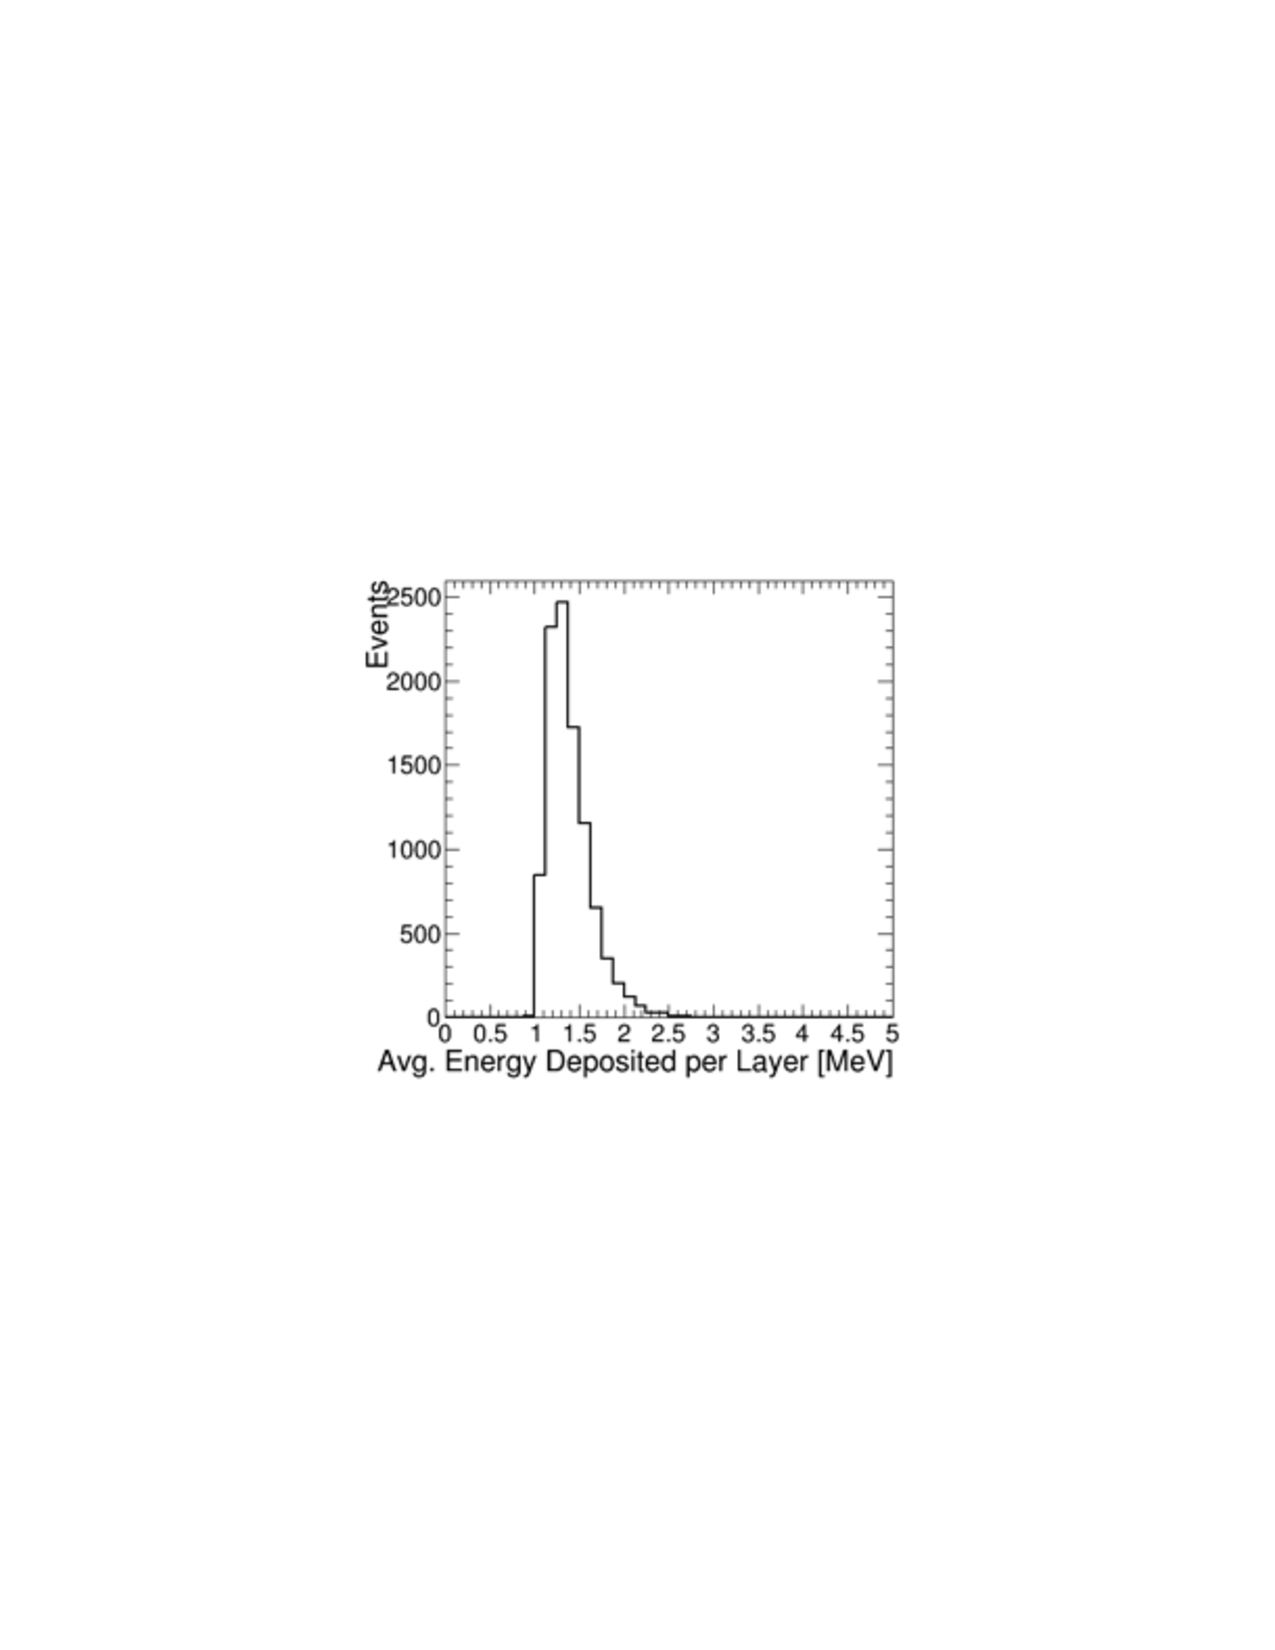
\includegraphics[width=0.5\textwidth]{images/hcal_mip.pdf}
    \caption{Distribution of energies deposited in scintillator from muon to characterize MIP behavior in plastic scintillator}
 \label{fig:hcalMIP}
 \end{center}
\end{figure}
